\documentclass[conference]{IEEEtran}

\usepackage{cite}
\usepackage{amsmath,amssymb,amsfonts}
\usepackage{algorithmic}
\usepackage{graphicx}
\usepackage{textcomp}
\usepackage{xcolor}
\usepackage{hyperref}
\usepackage{booktabs}
\usepackage{float} % in the preamble
\usepackage{url}
\usepackage{hyperref}
 
\def\BibTeX{{\rm B\kern-.05em{\sc i\kern-.025em b}\kern-.08em
    T\kern-.1667em\lower.7ex\hbox{E}\kern-.125emX}}
    
\begin{document}

\title{Individual Project - Generative Scene Generation}

\author{\IEEEauthorblockN{Denis Topallaj}
\IEEEauthorblockA{\textit{Universiteit Hasselt} \\
Hasselt, Belgium \\
denis.topallaj@student.uhasselt.be}
}

\maketitle

\begin{abstract}
This is a brief and self-contained summary of the contents of your paper. Mention what you did and report very briefly on the most important findings. You should see this as a 'teaser' for reading the entire document. Do not include references or citations, and make sure nothing in your text refers back to the abstract. Your entire paper is not allowed to exceed 10 pages in length, including figures and tables, but excluding references!
\end{abstract}

\section{Introduction}

Recent advances in generative artificial intelligence have enabled remarkable progress in creating complex visual content from simple textual or visual prompts. Models such as Stable Diffusion, DALL·E~3, and Imagen have demonstrated the feasibility of translating text into realistic images, while emerging text-to-video and text-to-3D techniques extend these capabilities into the spatio-temporal domain. This rapid development opens new opportunities for automatic 3D content creation, an area traditionally dominated by manual modeling and time-intensive workflows.

Three-dimensional (3D) scene generation is a particularly challenging problem, as it requires not only plausible geometry but also coherent appearance and spatial consistency across multiple views. Recent methods such as Neural Radiance Fields (NeRF)~\cite{nerf_paper} and 3D Gaussian Splatting (3DGS)~\cite{3d_gaussian_splatting_paper} have provided efficient and high-quality representations for reconstructing and rendering real-world scenes from multi-view imagery. However, generating 3D content directly from text or single images remains an open challenge, as it requires synthesizing unseen viewpoints and consistent geometry without explicit supervision.

One promising approach to this challenge is to construct an indirect generative pipeline that first converts a text or image prompt into a short video sequence, which is then used as input for 3D reconstruction methods such as Gaussian Splatting. This intermediate video stage provides multiple viewpoints of the same scene, improving multi-view consistency and enabling reconstruction-based 3D methods to operate more effectively. Alternatively, emerging models such as WorldGen~\cite{worldgen_site} and MVDream~\cite{mvdream_paper} attempt to generate 3D representations directly from text or image input, bypassing the need for intermediate video generation.

In this project, we explore and compare these different approaches to generative 3D scene creation. Specifically, we design a pipeline that takes text or image prompts as input and produces a 3D Gaussian Splatting representation of the resulting scene. We then compare this indirect pipeline (text/image-to-video-to-3DGS) with state-of-the-art direct text-to-3D methods in terms of quality, realism, efficiency, and reconstruction fidelity.

The central research question that guides this work is the following.

\begin{quote}
\emph{How do different generative pipelines based on text, images, or videos inputs affect the quality, realism, and efficiency of 3D scene reconstruction using Gaussian Splatting?}
\end{quote}

The remainder of this paper is structured as follows. Section~\ref{sec:relatedwork} reviews related work in generative 3D modeling and Gaussian Splatting. Section~\ref{sec:methodology} describes the design of the proposed pipeline and the comparison framework. Section~\ref{sec:implementation} details the practical implementation setup. Section~\ref{sec:results} presents the experimental results and evaluation, followed by a discussion in Section~\ref{sec:discussion}. Finally, Section~\ref{sec:conclusion} concludes the article and outlines potential directions for future research.

\section{Related Work}
\label{sec:relatedwork}

In recent years, generative methods for 3D reconstruction and scene synthesis have advanced rapidly. 
This section reviews the most relevant developments, starting from neural scene representations such as Neural Radiance Fields (NeRF) and 3D Gaussian Splatting (3DGS), followed by an overview of direct text-to-3D methods and text-to-video generation approaches that form the foundation for this work.

\subsection{Neural Radiance Fields (NeRF)}

Neural Radiance Fields (NeRF)~\cite{nerf_paper} represent a breakthrough approach to 3D scene representation and novel view synthesis. It uses deep learning to encode a continuous volumetric scene representation, enabling photorealistic rendering of complex scenes from arbitrary viewpoints using only a sparse set of input images.

\subsubsection{Core Concept}
At its foundation, NeRF models a static scene as a continuous 5D function that maps a 3D spatial location $x = (x, y, z)$ and a 2D viewing direction $d = (\theta, \phi)$ to a volume density $\sigma$ and view-dependent emitted radiance $(color)\:c = (r, g, b)$. This function is approximated by a multilayer perceptron (MLP), a type of fully connected neural network that learns to represent the scene through optimization.~\cite{nerf_paper_p1}. The MLP model overfits on the data points provided, trying to achieve a 1:1 ratio on the images.

The key insight is that by querying this function at various points along camera rays and using classical volume rendering techniques, NeRF can synthesize novel views of the scene with remarkable fidelity, capturing complex lighting effects, occlusions, and fine geometric details.~\cite{nerf_paper_p5}

\begin{figure}[H]
    \centering
    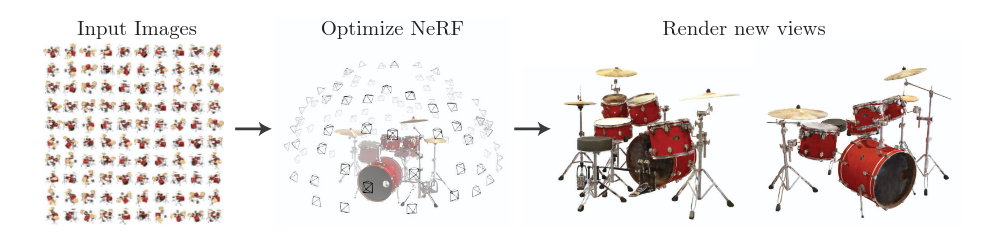
\includegraphics[width=1\linewidth]{nerf-drums-example.png}
    \caption{NeRF Drums Example ~\cite{nerf_paper_p2}}
    \label{fig:nerf-drums}
\end{figure}

The synthetic Drums scene comprises 100 input views, each randomly positioned on a hemisphere surrounding the object. Visualizing these views helps illustrate NeRF’s novel view synthesis capabilities: after training, two new perspectives are rendered from the optimized scene representation. To render an image from a particular viewpoint, the process unfolds as follows.
\begin{itemize}
    \item Camera rays are cast through every pixel, generating sampled points in 3D space along each ray.
    \item The neural network receives these 3D coordinates along with their corresponding 2D viewing directions, outputting color and density values for each point.
    \item Classical volume rendering techniques aggregate these values, converting the samples into a final 2D image.
\end{itemize}
Since this entire pipeline is differentiable, gradient descent can be used to optimize the parameters of the NeRF model. By minimizing the discrepancy between observed images and images synthesized by the model, the network is trained to assign coherent densities and colors, faithfully representing the true underlying content across multiple viewpoints. ~\cite{nerf_paper_p2}

\subsubsection{Spatial Encoding Network}
The first part of the MLP takes as input a 3D position $x$ and outputs the volume density $\sigma$ and a 256-dimensional feature vector. The volume density $\sigma$ represents how much light is absorbed or scattered at that point in space. The higher the value, the more opaque the region. This density is predicted independently of the viewing direction, imposing geometric consistency in different viewpoints.~\cite{nerf_paper_p5}

\begin{figure}[H]
    \centering
    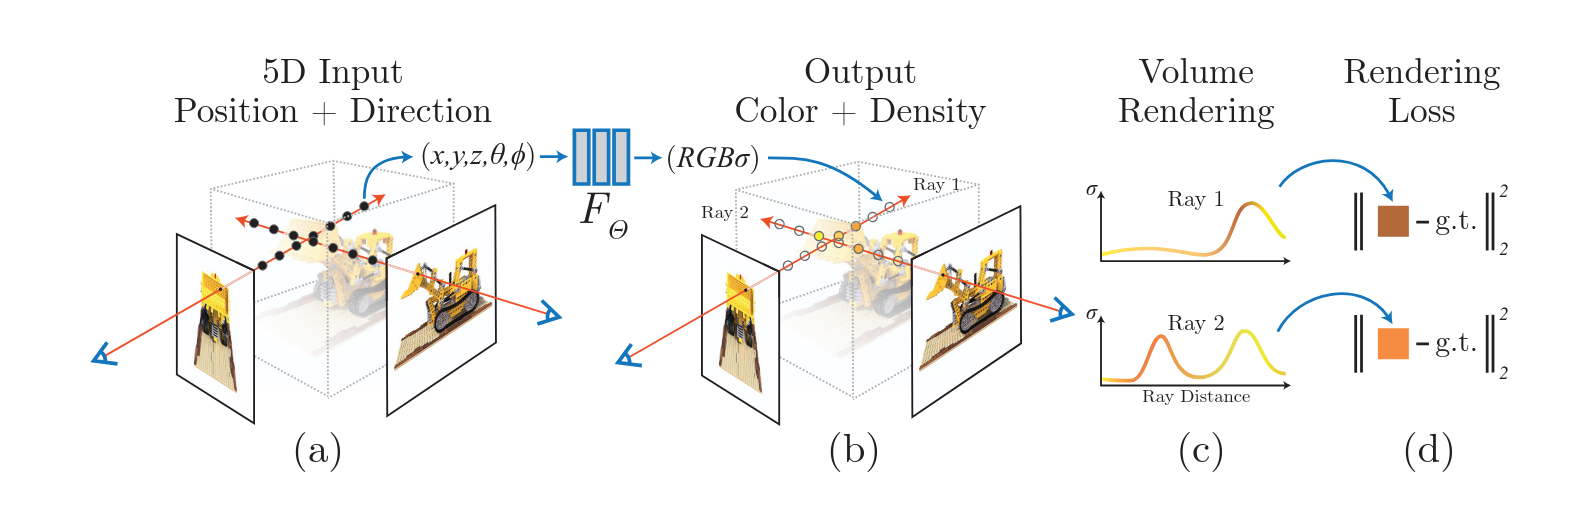
\includegraphics[width=1\linewidth]{spatial-encoding-network.png}
    \caption{Spacial Encoding Network ~\cite{nerf_paper_p5}}
    \label{fig:spacial_encoding_network}
\end{figure}

The following is an overview of the neural radiance field scene representation and differentiable rendering procedure:
\begin{itemize}
    \item Sample 5D coordinates consisting of spatial location and viewing direction along each camera ray to represent how light interacts with the scene.
    \item Using these values as input for an MLP to predict a color and volume density.
    \item The color and density values are combined using volume rendering techniques, integrating contributions along the ray to form a synthesized image.
    \item The network can be trained by minimizing the residual error between the rendered images and the real ground truth observations, since the rendering process is differential. ~\cite{nerf_paper_p5}
\end{itemize}

\subsubsection{View-Dependent Color Network}

The 256-dimensional feature vector from the first network is concatenated with the viewing direction $d$ and passed through additional layers to predict the $RGB\;color\;c$. This separation allows the network to model view-dependent appearance effects such as reflections and glossy surfaces, where the observed color changes based on the viewing angle. ~\cite{nerf_paper_p6}

\subsubsection{Positional Encoding}

NeRF's success lies with the use of positional encoding applied to the input coordinates. Using raw 3D coordinates and viewing directions are transformed using high-frequency sinusoidal functions of the form: $\gamma(p) = (\sin{2^0 \pi p}, \cos{(2^0 \pi p)}, ..., \sin{2^{L-1} \pi p}, \cos{(2^{L-1} \pi p)})$.~\cite{nerf_paper_p7}

$L$ represents the number of frequency levels (or octaves) used in positional encoding. When the function $\gamma(p)$ is applied, it creates sine and cosine functions at different frequencies. The parameter $L$ determines how many different frequencies it can use, ranging from $2^0\pi$ to $2^{L-1}\pi$. Typically, $L=10$ is used in NeRF for spatial coordinates (60 total encoded dimensions) and $L=4$ for viewing directions (16 total encoded dimensions).~\cite{nerf_paper_p7}~\cite{nerf_paper_p8}

The reason $L=10$ is used for positions and $L=4$ for directions is that spatial positions need to capture finer details (high-frequency information such as sharp edges and textures), while viewing directions require less granularity since lighting and appearance changes are typically smoother.~\cite{nerf_paper_p7}~\cite{nerf_paper_p8}

This encoding maps the input to a higher-dimensional space and enables the network to learn high-frequency details in the scene. Without this encoding, the MLP would struggle to represent fine textures and sharp angles or boundaries due to the spectral bias of neural networks toward learning lower-frequency functions.~\cite{nerf_paper_p8}

\subsubsection{Hierarchical Sampling Strategy}

NeRF employs a two-stage hierarchical sampling approach to improve rendering efficiency. A "coarse" network first samples points uniformly along each ray. Based on the predicted density values from this coarse network, a second "fine" network samples additional points concentrated in regions more likely to contain visible geometry. This stratified sampling strategy allocates more computational resources to relevant parts of the scene, improving both quality and efficiency.~\cite{nerf_paper_p8}

\subsubsection{Limitations}

Despite its impressive capabilities, NeRF has notable limitations:

\begin{itemize}
    \item Long training times: Optimizing the network for a single scene can take hours to days.
    \item Slow rendering: Generating each image requires querying the network hundreds of thousands to millions of times.
    \item Static scenes only: The original formulation cannot handle dynamic objects or scene changes
    \item Many input views required: Typically requires 50-100 well-distributed input images for good results
    \item Difficulty with unbounded scenes: Performance degrades for large-scale outdoor environments without modifications
\end{itemize}~\cite{nerf_paper_p13}

These limitations have spawned extensive follow-up research addressing training speed, rendering efficiency, dynamic scenes, and generalization across multiple scenes, making NeRF a foundational technique in neural rendering and 3D vision. A comprehensive survey describing advances in 3D generation can be found here: \url{https://arxiv.org/pdf/2401.17807v1}.

\subsection{3D Gaussian Splatting}

In 2023 there was a paradigm shift in radiance field rendering. 3D Gaussian Splatting offers real-time performance while maintaining high visual quality. This method addresses the fundamental limitation of NeRF: the trade-off between rendering speed and visual quality. Unlike NeRF's implicit neural representation, 3D Gaussian Splatting uses an explicit scene representation based on millions of anisotropic 3D Gaussians, enabling real-time rendering at 30+ frames per second at 1080p resolution while achieving state-of-the-art visual quality.~\cite{3d_gaussian_splatting_paper}

\subsubsection{Core Concept}

The fundamental idea behind 3D Gaussian Splatting is to represent a 3D scene as a collection of oriented 3D Gaussian primitives distributed throughout space. Each Gaussian can be thought of as an ellipsoidal "blob" with specific properties that define its appearance and spatial extent. Rather than using a neural network to implicitly encode the scene as NeRF does, 3DGS explicitly stores these primitives and renders them through a differentiable rasterization process.

This explicit representation offers several key advantages: it avoids sampling empty space during rendering, provides direct control over scene elements, and leverages GPU rasterization hardware for efficient rendering. The scene can be rendered by projecting these 3D Gaussians onto the image plane and compositing them in a visible manner.~\cite{3d_gaussian_splatting_paper_p2}

\subsubsection{Gaussian Primitive Representation}

Each 3D Gaussian in the scene is characterized by a set of learnable parameters that fully define its spatial properties:

\begin{itemize}
    \item Position (mean) $\mu$: A 3D vector $(x, y, z)$ defines the center of the Gaussian in world space.
    \item Covariance matrix $\sum$: A $3 \times 3$ matrix that defines the shape and orientation of the Gaussian ellipsoid, representing how the Gaussian extends in different directions
\end{itemize} ~\cite{3d_gaussian_splatting_paper_p4}

The covariance matrix is crucial for representing anisotropic structures. Gaussians can be elongated in specific directions to efficiently model thin structures such as edges, surfaces, and fine details. This anisotropy is a key factor in achieving high-quality reconstruction with fewer primitives. The opacity $\alpha$ is a scalar value in $[0,1]$ representing the transparency of the Gaussian, and the color is represented using spherical harmonic coefficients (explained in the next section) of varying degrees.~\cite{3d_gaussian_splatting_paper_p4}

\subsubsection{Spherical Harmonics for View-Dependent Color}

In 3D Gaussian Splatting, spherical harmonics are used to encode view-dependent color, enabling the appearance of each Gaussian to change realistically with the viewing direction. Instead of representing colors as simple RGB values, each Gaussian stores a set of coefficients corresponding to spherical harmonic (SH) basis functions. When rendering, the color observer from a particular viewing direction is computed by evaluating these SH basis functions for that direction and taking a weighted sum using the stored coefficients.~\cite{3d_gaussian_splatting_paper_p3}~\cite{towards_data_science_gaussian_splatting}

This allows the color to capture complex effects like specular highlights and gloss that vary with view angle, rather than being fixed per point. For example, low-order SHs can smoothly interpolate diffuse color changes, while higher orders can encode more detailed view-dependent phenomena. In practice, the implementation typically uses SH of a degree up to three, balancing expressiveness with computational cost.~\cite{3d_gaussian_splatting_paper_p3}~\cite{3d_gaussian_splatting_paper_p4}

\subsubsection{Rendering and Optimization}

The rendering pipeline projects 3D Gaussians onto the 2D image plane using a tile-based rasterization approach. The screen is divided into $16 \times 16$ pixel tiles, with Gaussians sorted by depth within each tile. For each pixel, the final color is computed through alpha blending in front-to-back order: The pixel color is computed as $C = \sum_i^N T_i\alpha_ic_i$, where $T_i$ is the accumulated transmittance and $c_i$ is the color at each sample. The opacity term $\alpha_i = (1-\exp(-\sigma_i\delta_i))$ is derived from the volume density $\sigma_i$ and sampling interval $\delta_i$. Rendering stops once accumulated opacity exceeds 0.9999.~\cite{3d_gaussian_splatting_paper_p3}~\cite{3d_gaussian_splatting_paper_p6}~\cite{3d_gaussian_splatting_paper_p14}

3DGS initializes from Structure-from-Motion (SfM) points and employs adaptive density control during optimization. Under-reconstructed regions are densified through \textit{cloning} (copying small Gaussians) or \textit{splitting} (dividing large Gaussians), while \textit{pruning} removes low-opacity or oversized Gaussians every 100 iterations. The optimization minimizes $\mathcal{L} = (1 - \lambda)\mathcal{L}_1 + \lambda\mathcal{L}_{\text{D-SSIM}}$ with $\lambda = 0.2$, converging in 7,000--30,000 iterations (minutes to hours) compared to NeRF's multi-day training.~\cite{3d_gaussian_splatting_paper_p5}~\cite{3d_gaussian_splatting_paper_p6}

\begin{figure}[H]
    \centering
    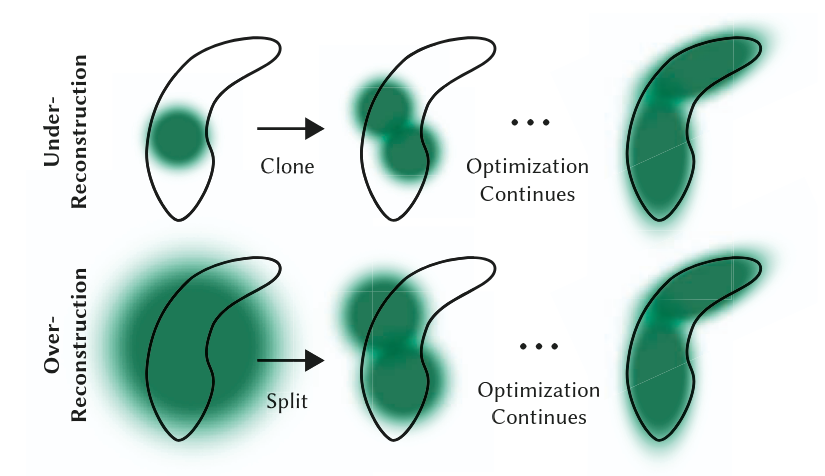
\includegraphics[width=1\linewidth]{gaussians-optimization.png}
    \caption{Gaussians Optimization ~\cite{3d_gaussian_splatting_paper_p6}}
    \label{fig:gaussians-optimization}
\end{figure}

\subsubsection{Advantages and Limitations}

Compared to NeRF, 3DGS offers real-time rendering (30+ FPS at 1080p), 10--100× faster training, explicit scene representation enabling direct manipulation, and efficient handling of fine details through anisotropic Gaussians. However, it requires significant GPU memory for millions of Gaussians, depends on quality SfM initialization, and can produce "floater" artifacts without proper regularization. Like NeRF, it assumes static scenes and quality degrades for views far from training cameras.~\cite{3d_gaussian_splatting_paper_p2}~\cite{3d_gaussian_splatting_paper_p10}~\cite{3d_gaussian_splatting_paper_p11}


\section{Methodology}
\label{sec:methodology}

This section describes how 3D environments can be generated from text, image, and video inputs, and outlines the pipelines explored in this project. The fundamental challenge in generative 3D scene creation is that text and images are inherently 2D signals, yet 3D reconstruction methods such as Gaussian Splatting require geometrically consistent multi-view observations. The approaches surveyed here differ primarily in \textit{how} they bridge this gap: either by generating 3D structure directly, or by using an intermediate representation (video) to synthesize the multi-view observations needed for reconstruction.

\subsection{Direct Text/Image-to-3D Generation}

Direct methods attempt to produce a 3D representation in a single end-to-end pipeline without requiring an explicit intermediate video step. These methods are appealing because they avoid error propagation across pipeline stages and can enforce geometric consistency by design.

WorldGen~\cite{worldgen_site} is one such system, operating in two stages. In the first stage, a high-resolution 360° panorama is synthesized from the input text or image prompt. This panorama captures the global layout and appearance of the entire scene in a single equirectangular image, providing a holistic view that inherently encodes spatial relationships between scene elements. In the second stage, this panorama is lifted into a full 3D scene by converting it into either a 3D Gaussian Splatting or mesh representation, enabling free 360° exploration with loop closure consistency.~\cite{worldgen_site} The key insight behind this two-stage design is the decoupling of global scene layout generation from per-point geometry estimation. Generating a panorama first constrains the overall structure of the scene before any 3D lifting is attempted, which helps maintain global coherence. Because both stages are highly optimized, WorldGen can produce explorable 3D scenes in a matter of seconds, making it one of the fastest approaches currently available.

\begin{figure}[H]
    \centering
    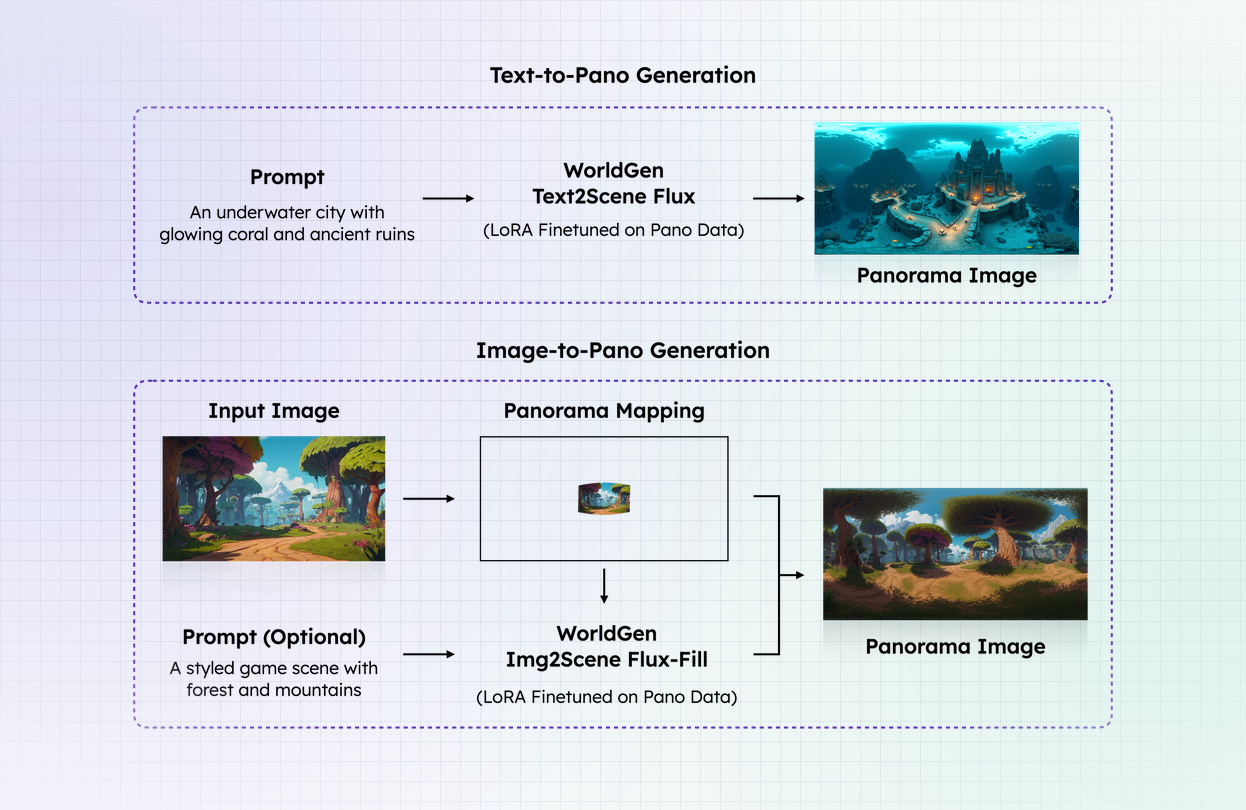
\includegraphics[width=1\linewidth]{worldgen-pipeline.png}
    \caption{world.gen ~\cite{worldgen_site}}
    \label{fig:world-gen-pipeline}
\end{figure}

MVDream~\cite{mvdream_paper} takes a complementary approach by training a multi-view diffusion model that jointly synthesizes several geometrically consistent views of a scene from a single text prompt. Conventional text-to-image diffusion models generate each view independently, with no mechanism to enforce that the same geometry is depicted across frames. MVDream addresses this by conditioning the denoising process across multiple camera viewpoints simultaneously, sharing attention across views so that the model learns to produce consistent geometry and appearance. The resulting multi-view images can then be used directly to initialize a 3D reconstruction pipeline such as 3DGS, making MVDream a strong and controllable baseline for text-to-3D generation.~\cite{mvdream_paper} Because the viewpoints are specified explicitly as conditioning inputs, the user retains meaningful control over the coverage of the reconstructed object or scene, which is a notable advantage over methods where camera trajectories are implicit.

\begin{figure}[H]
    \centering
    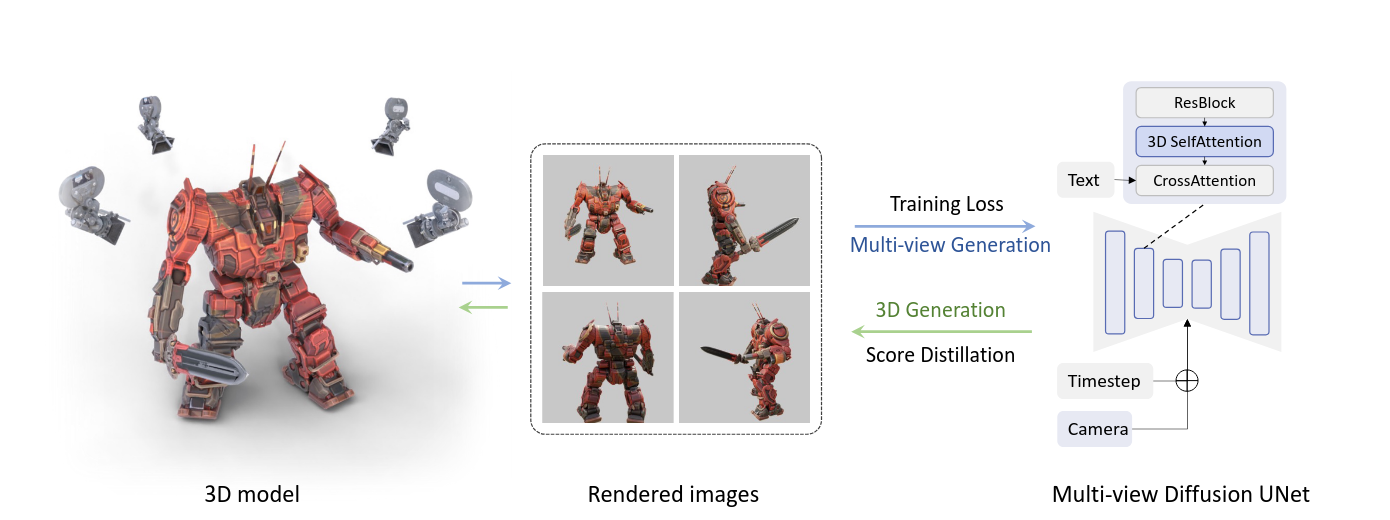
\includegraphics[width=1\linewidth]{mvdream-example.png}
    \caption{MVDream ~\cite{mvdream_paper_p3}}
    \label{fig:mvdream-example}
\end{figure}

A general limitation shared by direct methods is that they must learn the mapping from 2D signals to 3D geometry entirely from training data. This means their generalization is bounded by the diversity of 3D scenes seen during training, and they can struggle with highly novel or out-of-distribution prompts. Producing large-scale, unbounded outdoor scenes remains particularly difficult for direct approaches.

\subsection{Indirect Pipeline: Text/Image $\rightarrow$ Video $\rightarrow$ 3DGS}

An alternative strategy is to use a text-to-video or image-to-video model as an intermediate step. Rather than generating 3D structure directly, a short video clip is first synthesized from the input prompt. This video implicitly provides a sequence of frames depicting the scene from varying viewpoints, which can then be treated as a pseudo-multi-view capture and passed into a 3D Gaussian Splatting reconstruction pipeline.

The reconstruction stage first estimates camera poses for each extracted frame, typically using a Structure-from-Motion (SfM) algorithm such as COLMAP, which identifies feature correspondences across frames and solves for the camera trajectory. Once poses are known, the 3DGS optimization is initialized from the sparse SfM point cloud and refined to minimize the photometric error across all input frames, exactly as it would be for a real-world capture scenario.

This indirect approach has several compelling advantages. Text-to-video models have been trained on enormous collections of real-world footage and can generate temporally coherent, photorealistic content across a wide variety of scenes and styles. By leveraging this prior knowledge, the indirect pipeline can generalize to a broad range of prompts without requiring any 3D-specific training data. Furthermore, because the 3DGS reconstruction stage operates on the generated frames in the same way it would on real photographs, improvements in either the video generation model or the reconstruction algorithm can be incorporated independently.

However, the indirect pipeline also inherits the limitations of each stage. Video generation models do not explicitly control the camera trajectory: the synthesized motion may be too limited, too erratic, or insufficiently diverse to provide the viewpoint coverage that 3DGS reconstruction requires. Multi-view consistency is not guaranteed since the video model has no explicit 3D representation, meaning that fine geometric details can change between frames in ways that are visually plausible but geometrically contradictory. Such inconsistencies manifest as floaters, blurring, or incomplete geometry in the final reconstruction. Additionally, any systematic artifact in the generated video (such as over-smoothed textures, temporal flicker, or incorrect lighting) will propagate directly into the 3D scene.

\subsection{Pipeline Overview: Text/Image $\rightarrow$ Video $\rightarrow$ 3DGS}

The pipeline implemented in this project takes a text or image prompt as input and produces an explorable 3D Gaussian Splatting scene as output, using video generation as an intermediate step. The pipeline consists of three sequential stages.

In the first stage, a text-and-image-to-video model synthesizes multiple short video clips from the input prompt, which are composed into an orbital trajectory around the scene. Models such as Wan2.1~\cite{wan_paper} and Wan2.2~\cite{wan_paper} support camera motion conditioning, allowing each clip to be guided by a specific directional prompt (e.g. pan left, pan right, tilt up) while remaining anchored to the same reference image. By generating clips along complementary directions --- horizontal pans, vertical tilts, and diagonal arcs --- and stitching them together, the combined sequence approximates a full orbital path around the scene. Anchoring every clip to the same reference image maintains visual consistency across clips, ensuring that the merged video depicts a coherent scene rather than a collection of unrelated viewpoints. The clips are ordered and concatenated to form a single continuous video with smooth transitions, which is passed to the second stage.

In the second stage, camera poses are estimated for each extracted video frame using Structure-from-Motion. Feature correspondences are identified across frames and used to solve for the camera positions and orientations, while simultaneously producing a sparse 3D point cloud of the scene. The quality of this pose estimation is critical: inaccurate poses will cause the subsequent reconstruction to diverge or produce blurred geometry, so only frames with reliable pose estimates are retained. Because SfM relies on finding shared features across clip boundaries, smooth transitions between clips are essential for this stage to succeed.

In the third stage, the extracted frames and their estimated camera poses are passed into a 3D Gaussian Splatting reconstruction pipeline. The Gaussian primitives are initialized from the sparse SfM point cloud and optimized over thousands of iterations to minimize the photometric error across all input frames, as described in Section~\ref{sec:relatedwork}. The result is a fully explorable 3D scene that can be rendered from arbitrary novel viewpoints in real time.

The primary challenge of this pipeline lies in the imperfect nature of generated video as a substitute for real multi-view capture. Unlike a physical camera orbiting a real scene, the video model has no explicit 3D representation: it hallucinates plausible frames conditioned on motion prompts, which means geometric details can subtly shift between clips even when anchored to the same reference image. The following section describes the specific tools and models chosen for each stage, and the practical measures taken to mitigate these inconsistencies.

\section{Implementation}
\label{sec:implementation}

This section describes the practical realisation of the generative 3D scene generation pipeline. The implementation encompasses five tightly coupled components: a video generation stage powered by a pretrained generative model, a containerised execution environment, a Structure-from-Motion preprocessing pipeline, a 3D Gaussian Splatting training application, and a web-based user interface that ties the full workflow together. Each component is described in turn, together with the rationale for the technical choices made.

\subsection{Development Environment and Containerisation}

A central challenge in GPU-accelerated computer vision research is the fragility of the software environment: CUDA versions, driver compatibility, and library ABIs must all align precisely for the code to compile and run correctly. To eliminate this source of variability, the entire project is packaged inside a Docker container based on the official NVIDIA CUDA image, parameterised by the CUDA version at build time. This allows the same container definition to be reused across different GPU generations without modification.

The container installs all system dependencies required by both the C++ application and the Python frontend: X11 development libraries for OpenGL display, a GCC 14 toolchain, Python with virtual-environment support, and a modern CMake release sourced directly from Kitware. A dedicated Python virtual environment is provisioned inside the image with the Gradio library, isolating Python dependencies from the system interpreter. User-level isolation is achieved by propagating the host user's UID, GID, and username into the container at build time, so that files created inside the container are owned correctly on the host filesystem.

The Docker Compose configuration maps the project source tree into the container with a bind mount, forwards the X11 socket and Xauthority cookie for OpenGL rendering, and grants the container access to all NVIDIA GPUs. Memory is capped at 24~GB to prevent runaway allocations during Gaussian Splatting optimisation. Inter-process communication and PID namespaces are shared with the host, which is required for CUDA's unified virtual memory to function correctly across process boundaries.

Because COLMAP requires GPU access even in offscreen mode through the OpenGL context it creates internally, the host X11 display server must be made accessible to the container before launching it. A helper script wraps the Docker Compose commands and handles this setup step.

\subsection{Video Generation with Wan2GP and LTX Video}

The first stage of the pipeline produces the input video from which the 3D scene is later reconstructed. This is accomplished using Wan2GP~\cite{wan2gp_site}, an open-source graphical interface available on GitHub that provides access to a wide range of text-to-video and image-to-video generative models through a Gradio-based web interface. For this project the LTX Video model~\cite{ltxvideo_paper} is used as the generative backbone.

The core challenge in using a video model for 3D reconstruction is multi-view consistency: independently generated frames may depict the same scene in locally plausible but geometrically contradictory ways, causing COLMAP to fail at matching features across frames or producing an incoherent sparse point cloud. To address this, Wan2GP supports image-anchored generation, where one or more reference images are provided alongside the text prompt and the model is conditioned to begin and end each clip at those frames. By anchoring every generated clip to the same reference image of the scene, the model is constrained to maintain a consistent appearance and overall geometry across clips, even when the camera direction changes between them.

In practice, a text prompt describing the desired scene and a reference image generated by a text-to-image model are provided as input. Multiple short video clips are generated, each conditioned on a directional motion prompt (for example, panning left, panning right, or tilting upward) and anchored to the same reference frame. The clips are then concatenated into a single video that approximates an orbital path around the scene. This combined video is passed as input to the COLMAP pipeline described in the next subsection.

\subsection{LichtFeld-Studio: 3D Gaussian Splatting Training and Visualisation}

The third stage performs the actual 3D Gaussian Splatting reconstruction using LichtFeld-Studio~\cite{lichtfeld_studio_site}, an open-source C++ application published on GitHub. LichtFeld-Studio implements Gaussian Splatting training, real-time rendering, and interactive scene visualisation in a single executable. For this project the application is integrated as-is, with additional shell scripts contributed at the repository level to automate the preprocessing and postprocessing steps, and targeted configuration adjustments to make training feasible on consumer-grade GPU hardware.

LichtFeld-Studio is built with CMake and the Ninja build system. Its dependencies are managed via vcpkg, which provisions all required C++ libraries from source to ensure reproducible builds. Key dependencies include GLFW and OpenGL for windowing and rendering, GLM for linear algebra, Dear ImGui for the graphical user interface, Intel TBB for CPU parallelism, OpenImageIO for image I/O, and a CUDA/PyTorch backend for the performance-critical rasterisation and gradient computation kernels. The build system automatically detects the GPU's compute capability and compiles CUDA kernels for the native architecture.

For this project the 3DGUT rendering backend~\cite{gut_paper} is used. 3DGUT, developed by NVIDIA Research, replaces the standard tile-based rasteriser with a ray-tracing-based renderer that correctly handles cameras with lens distortion models. Because the COLMAP pipeline estimates a distortion-aware camera model, using 3DGUT ensures that the distortion parameters are applied correctly during training. Without this, the rendered views would not match the training images and the optimisation would not converge to an accurate reconstruction.

LichtFeld-Studio also supports camera pose refinement during training, which compensates for small alignment errors introduced by COLMAP~\cite{3rgs_paper}. This is particularly valuable for the indirect pipeline, where the synthesised video frames may exhibit subtle geometric inconsistencies that cause COLMAP to produce slightly inaccurate pose estimates. A timelapse feature saves rendered checkpoints at regular intervals during training, allowing convergence to be inspected visually after the fact.

The training loop follows the original 3DGS formulation: Gaussian primitives initialised from the sparse COLMAP point cloud are optimised via gradient descent to minimise a weighted combination of $\mathcal{L}_1$ photometric loss and D-SSIM. Adaptive density control densifies under-reconstructed regions by cloning or splitting Gaussians and prunes low-opacity or oversized primitives periodically. The output is a PLY file containing the trained scene, which can be opened in any Gaussian Splatting viewer.

LichtFeld-Studio also bundles a Mip-NeRF~360 benchmark suite~\cite{mipnerf360_paper} that evaluates reconstruction quality against the standard reference dataset, using both the MCMC training strategy and the Adaptive Density Control strategy. These benchmarks provide the timing and quality figures used in Section~\ref{sec:results}.

\subsection{COLMAP Structure-from-Motion Pipeline}

The second stage of the pipeline processes the generated video into a set of calibrated camera poses and a sparse 3D point cloud, which together provide the initialisation required by the Gaussian Splatting training stage. This is handled by a self-contained Bash script that takes a video file as input and produces a COLMAP reconstruction suitable for direct ingestion by LichtFeld-Studio. The script accepts the path to the input video, a project directory name, and the frame extraction rate as parameters. A configurable cap on the total number of extracted frames prevents excessively large reconstructions on longer videos.

Frame extraction is performed by FFmpeg, which decodes the video and writes JPEG frames at the target rate. If the expected frame count would exceed the configured maximum, the extraction rate is automatically scaled down to stay within the limit. Near-lossless JPEG quality is used to preserve the fine structure needed for reliable feature detection.

SIFT feature extraction is performed by COLMAP in CPU-only mode. This departure from the GPU-accelerated default is necessary in the containerised environment, where COLMAP's internal OpenGL context creation for GPU feature extraction fails due to the interaction between the NVIDIA driver and the X11 forwarding setup. The camera model used includes radial and tangential distortion coefficients, which are estimated jointly with the camera intrinsics and later consumed by the 3DGUT renderer in LichtFeld-Studio.

Feature matching uses COLMAP's sequential matcher rather than the exhaustive matcher. Exhaustive matching has quadratic complexity in the number of frames and is designed for unordered image collections. Video frames are inherently sequential, so sequential matching, which compares each frame only against its nearest temporal neighbours, reduces matching time from $O(n^2)$ to $O(n \cdot k)$ while producing equivalent results for the orbital trajectory structure of the generated videos. Loop detection is disabled to avoid false positive loop closures in the synthesised camera paths. If an NVIDIA GPU is detected at runtime, it is used for the matching stage, which does not require an OpenGL context and therefore works reliably inside the container.

Sparse 3D reconstruction is then run with focal length and distortion refinement enabled. The resulting sparse model is verified by checking that a sufficient number of images were registered, then converted to the text format expected by LichtFeld-Studio, and finally the images are undistorted so that the training frames match the calibrated camera geometry. Dense reconstruction is available in the script but skipped by default, as Gaussian Splatting does not require a dense depth map for initialisation.

\subsection{Gradio Web Interface}

To make the reconstruction pipeline accessible without requiring manual command-line interaction, a web-based frontend was developed using the Gradio framework and served from within the Docker container. The interface presents users with three input controls: a video file upload widget, a text field for naming the output project directory, and a numeric control for the frame extraction rate. A single button triggers the full two-stage pipeline consisting of COLMAP preprocessing followed by LichtFeld-Studio training.

The backend processing function runs as a Python generator that streams incremental status messages to the frontend, providing real-time feedback during the long-running COLMAP and LichtFeld-Studio stages. To prevent the interface from becoming unresponsive under the volume of output produced by COLMAP, a selective logging filter retains only lines associated with errors, warnings, and major milestones such as feature extraction progress, registration counts, and stage completion. A periodic heartbeat message confirms that the process is still running during periods of low output. Terminal colour codes from the Bash scripts are stripped before display.

After both stages complete successfully, the function archives the COLMAP project directory and the LichtFeld-Studio output directory into a ZIP file and presents it as a downloadable file widget. The archive contains the sparse point cloud files, undistorted images, and the trained Gaussian Splatting model in PLY format. A graceful handler covers the case where the application exits with a segmentation fault after a successful training run, which occurs when the user closes the OpenGL window via the window manager rather than through the application's own quit mechanism.

\subsection{Quality Evaluation Framework}

A dedicated evaluation framework defines the metrics used to assess reconstruction quality. These fall into four categories: reference-based metrics that compare rendered views against held-out ground-truth photographs, no-reference metrics computed directly on rendered frames without a ground truth, geometric accuracy metrics that compare the Gaussian point cloud against the COLMAP sparse reconstruction, and depth accuracy metrics.

The reference-based metrics are Peak Signal-to-Noise Ratio (PSNR), Structural Similarity Index (SSIM), and Learned Perceptual Image Patch Similarity (LPIPS). PSNR measures pixel-level fidelity on a logarithmic decibel scale; scores above 30~dB indicate good reconstruction quality. SSIM assesses perceptual similarity through luminance, contrast, and local structure comparisons; values above~0.80 are considered good. LPIPS, computed using a neural network feature extractor trained on human perceptual judgements, provides the most human-aligned quality estimate; lower values indicate better perceptual similarity.

The no-reference metrics assess rendered frame quality without any ground truth: sharpness is measured via the Laplacian variance of the grayscale image, brightness via mean pixel intensity, and contrast via the standard deviation of pixel intensity. These metrics are particularly useful in the generative pipeline setting, where held-out real photographs do not exist for the AI-generated input data.

Geometric accuracy is quantified by the Chamfer distance between the Gaussian point cloud and the COLMAP sparse point cloud, measuring how closely the 3D structure of the splat matches the reference. Depth accuracy is characterised by the Absolute Relative Error (AbsRel) and Root Mean Squared Error (RMSE) of Z-coordinate depths, as well as the $\delta_1$, $\delta_2$, and $\delta_3$ threshold metrics, which report the fraction of depth predictions within multiplicative factors of 1.25, $1.25^2$, and $1.25^3$ of the reference.

\section{Results}
\label{sec:results}

\section{Discussions}
\label{sec:discussion}

\section{Evaluation}
\label{sec:evaluation}

\section{Conclusion}
\label{sec:conclusion}



\subsection{Inserting tables}

Make sure your tables are legible and have decent aesthetics. Avoid the use of vertical lines if possible. More information can be found at the following link : \url{https://www.inf.ethz.ch/personal/markusp/teaching/guides/guide-tables.pdf}.

\vspace{0.5cm}
\begin{tabular}{llr}
  \toprule
  First name & Last Name & Grade \\
  \midrule
  John & Doe & $7.5$ \\
  Richard & Miles & $2$ \\
  \bottomrule
  \end{tabular}

  \vspace{0.5cm}

  \begin{tabular}{llr}  
    \toprule
    \multicolumn{2}{c}{Item} \\
    \cmidrule(r){1-2}
    Animal    & Description & Price (\$) \\
    \midrule
    Gnat      & per gram    & 13.65      \\
          &    each     & 0.01       \\
    Gnu       & stuffed     & 92.50      \\
    Emu       & stuffed     & 33.33      \\
    Armadillo & frozen      & 8.99       \\
    \bottomrule
  \end{tabular}

  
\subsection{Inserting figures}

When including figures or pictures, make sure that the quality is decent (don't upscale small and low-quality JPEG files). Preferably use vector formats for rescaling. If you copy something from another source, make sure that the original source is clearly referenced/cited. Charts and schematic overviews should be self-produced and not simply copy/pasted. Captions for figures need to be self-explanatory, so don't just mention 'screenhot' or 'chart' as a caption. You may also choose to include figures that span both columns, however be aware that this eats into your page allowance.

\begin{figure}[tbp]
\centerline{\includegraphics{fig1.png}}
\caption{Example of a figure caption with some relevant explanations.}
\label{fig}
\end{figure}

\section{Other tips}\label{othertips}

\begin{itemize}
\item Do not alter the layout of this document. You may include other packages if needed, but you may not mess with page margins, white spaces, fonts or font sizes. 
\item Make sure that your sections all contain a decent amount of text. Do not go overboard in the number of sections and subsections. For a paper like this there should be no need for subsubsections. 
\item Avoid 'lonely' sections, i.e. don't have a 3.1 if there is no 3.2 
\item Proofread all text before handing in for review. Spelling and grammatical errors are easily discovered by human readers and tools, use them (and not the teaching team). 
\item Cite all extern work you mention, see also below.
\item If needed, you can subdivide the paper into multiple files. As long as it produces output consistent with this template.
\item This template is based on the IEEEtran class. You can refer to the relevant documents for more information if needed (but this is typically not the case).

\end{itemize}

\section*{Conclusions}

This section contains the conclusions about your work. It is not an abstract ! Mention your research questions and how you succeeded (or not) in answering them. Be self-critical and reflect upon your own work.

\section*{Acknowledgments}
The author expresses sincere gratitude to \textbf{Joren Michels} for his invaluable guidance and mentorship throughout the duration of this project. Special thanks also go to \textbf{Lode Jorissen} and \textbf{Nick Michiels} for their continuous availability, insightful feedback, and technical support whenever questions arose. Finally, the author wishes to thank his parents for their unwavering support and encouragement during this work.

\iffalse % REFERENCES COMMENT
\section*{References}

Please number citations consecutively within brackets \cite{b1}. The 
sentence punctuation follows the bracket \cite{b2}. Refer simply to the reference 
number, as in \cite{b3}---do not use ``Ref. \cite{b3}'' or ``reference \cite{b3}'' except at 
the beginning of a sentence: ``Reference \cite{b3} was the first $\ldots$''
\fi

\begin{thebibliography}{00}

\bibitem{nerf_paper} Ben Mildenhall, Pratul P. Srinivasan, Matthew Tancik,
Jonathan T. Barron, Ravi Ramamoorthi, Ren Ng, UC Berkeley, Google Research, and UC San Diego ``NeRF: Representing Scenes as Neural Radiance Fields for View Synthesis`` \emph{\url{https://arxiv.org/pdf/2003.08934}}, 2020.
\bibitem{3d_gaussian_splatting_paper} Kerbl, Bernhard and Kopanas, Georgios and Leimk{\"u}hler, Thomas and Drettakis, George, ``3D Gaussian Splatting for Real-Time Radiance Field Rendering`` \emph{\url{https://repo-sam.inria.fr/fungraph/3d-gaussian-splatting/3d_gaussian_splatting_high.pdf}}, 2023.
% WORLDGEN SITE
\bibitem{worldgen_site} Ziyang Xie, ``WorldGen: Generate Any 3D Scene in Seconds`` \emph{\url{https://github.com/ZiYang-xie/WorldGen}}, 2025.
% MVDREAM PAPER
\bibitem{mvdream_paper} Yichun Shi, Peng Wang, Jianglong Ye, Long Mai, Kejie Li, Xiao Yang, ``MVDREAM: MULTI-VIEW DIFFUSION FOR 3D GENERATION`` \emph{\url{https://arxiv.org/pdf/2308.16512}}, 2024
\bibitem{mvdream_paper_p3} Yichun Shi, Peng Wang, Jianglong Ye, Long Mai, Kejie Li, Xiao Yang, ``MVDREAM: MULTI-VIEW DIFFUSION FOR 3D GENERATION`` \emph{\url{https://arxiv.org/pdf/2308.16512}}, 2024, pp.~3
% WAN PAPER
\bibitem{wan_paper} Team Wan, Ang Wang, Baole Ai, Bin Wen, Chaojie Mao, Chen-Wei Xie, Di Chen, Feiwu Yu, Haiming Zhao, Jianxiao Yang, Jianyuan Zeng, Jiayu Wang, Jingfeng Zhang, Jingren Zhou, Jinkai Wang, Jixuan Chen, Kai Zhu, Kang Zhao, Keyu Yan, Lianghua Huang, Mengyang Feng, Ningyi Zhang, Pandeng Li, Pingyu Wu, Ruihang Chu, Ruili Feng, Shiwei Zhang, Siyang Sun, Tao Fang, Tianxing Wang, Tianyi Gui, Tingyu Weng, Tong Shen, Wei Lin, Wei Wang, Wei Wang, Wenmeng Zhou, Wente Wang, Wenting Shen, Wenyuan Yu, Xianzhong Shi, Xiaoming Huang, Xin Xu, Yan Kou, Yangyu Lv, Yifei Li, Yijing Liu, Yiming Wang, Yingya Zhang, Yitong Huang, Yong Li, You Wu, Yu Liu, Yulin Pan, Yun Zheng, Yuntao Hong, Yupeng Shi, Yutong Feng, Zeyinzi Jiang, Zhen Han, Zhi-Fan Wu, Ziyu Liu ``WAN: OPEN AND ADVANCED LARGE-SCALE VIDEO GENERATIVE MODELS`` \emph{\url{arxiv.org/pdf/2503.20314}}, 2025
% NERF PAPER PAGES SOURCES
\bibitem{nerf_paper_p1} Ben Mildenhall, Pratul P. Srinivasan, Matthew Tancik,
Jonathan T. Barron, Ravi Ramamoorthi, Ren Ng, UC Berkeley, Google Research, and UC San Diego ``NeRF: Representing Scenes as Neural Radiance Fields for View Synthesis`` \emph{\url{https://arxiv.org/pdf/2003.08934}}, 2020, pp.~1
\bibitem{nerf_paper_p2} Ben Mildenhall, Pratul P. Srinivasan, Matthew Tancik,
Jonathan T. Barron, Ravi Ramamoorthi, Ren Ng, UC Berkeley, Google Research, and UC San Diego ``NeRF: Representing Scenes as Neural Radiance Fields for View Synthesis`` \emph{\url{https://arxiv.org/pdf/2003.08934}}, 2020, pp.~2
\bibitem{nerf_paper_p5} Ben Mildenhall, Pratul P. Srinivasan, Matthew Tancik,
Jonathan T. Barron, Ravi Ramamoorthi, Ren Ng, UC Berkeley, Google Research, and UC San Diego ``NeRF: Representing Scenes as Neural Radiance Fields for View Synthesis`` \emph{\url{https://arxiv.org/pdf/2003.08934}}, 2020, pp.~5
\bibitem{nerf_paper_p6} Ben Mildenhall, Pratul P. Srinivasan, Matthew Tancik,
Jonathan T. Barron, Ravi Ramamoorthi, Ren Ng, UC Berkeley, Google Research, and UC San Diego ``NeRF: Representing Scenes as Neural Radiance Fields for View Synthesis`` \emph{\url{https://arxiv.org/pdf/2003.08934}}, 2020, pp.~6
\bibitem{nerf_paper_p7} Ben Mildenhall, Pratul P. Srinivasan, Matthew Tancik,
Jonathan T. Barron, Ravi Ramamoorthi, Ren Ng, UC Berkeley, Google Research, and UC San Diego ``NeRF: Representing Scenes as Neural Radiance Fields for View Synthesis`` \emph{\url{https://arxiv.org/pdf/2003.08934}}, 2020, pp.~7
\bibitem{nerf_paper_p8} Ben Mildenhall, Pratul P. Srinivasan, Matthew Tancik,
Jonathan T. Barron, Ravi Ramamoorthi, Ren Ng, UC Berkeley, Google Research, and UC San Diego ``NeRF: Representing Scenes as Neural Radiance Fields for View Synthesis`` \emph{\url{https://arxiv.org/pdf/2003.08934}}, 2020, pp.~8
\bibitem{nerf_paper_p13} Ben Mildenhall, Pratul P. Srinivasan, Matthew Tancik,
Jonathan T. Barron, Ravi Ramamoorthi, Ren Ng, UC Berkeley, Google Research, and UC San Diego ``NeRF: Representing Scenes as Neural Radiance Fields for View Synthesis`` \emph{\url{https://arxiv.org/pdf/2003.08934}}, 2020, pp.~13
% 3D GAUSSIAN SPLATTING PAPER PAGES SOURCES
\bibitem{3d_gaussian_splatting_paper_p2} Kerbl, Bernhard and Kopanas, Georgios and Leimk{\"u}hler, Thomas and Drettakis, George, ``3D Gaussian Splatting for Real-Time Radiance Field Rendering`` \emph{\url{https://repo-sam.inria.fr/fungraph/3d-gaussian-splatting/3d_gaussian_splatting_high.pdf}}, 2023, pp.~2
\bibitem{3d_gaussian_splatting_paper_p3} Kerbl, Bernhard and Kopanas, Georgios and Leimk{\"u}hler, Thomas and Drettakis, George, ``3D Gaussian Splatting for Real-Time Radiance Field Rendering`` \emph{\url{https://repo-sam.inria.fr/fungraph/3d-gaussian-splatting/3d_gaussian_splatting_high.pdf}}, 2023, pp.~3
\bibitem{3d_gaussian_splatting_paper_p4} Kerbl, Bernhard and Kopanas, Georgios and Leimk{\"u}hler, Thomas and Drettakis, George, ``3D Gaussian Splatting for Real-Time Radiance Field Rendering`` \emph{\url{https://repo-sam.inria.fr/fungraph/3d-gaussian-splatting/3d_gaussian_splatting_high.pdf}}, 2023, pp.~4
\bibitem{3d_gaussian_splatting_paper_p5} Kerbl, Bernhard and Kopanas, Georgios and Leimk{\"u}hler, Thomas and Drettakis, George, ``3D Gaussian Splatting for Real-Time Radiance Field Rendering`` \emph{\url{https://repo-sam.inria.fr/fungraph/3d-gaussian-splatting/3d_gaussian_splatting_high.pdf}}, 2023, pp.~5
\bibitem{3d_gaussian_splatting_paper_p6} Kerbl, Bernhard and Kopanas, Georgios and Leimk{\"u}hler, Thomas and Drettakis, George, ``3D Gaussian Splatting for Real-Time Radiance Field Rendering`` \emph{\url{https://repo-sam.inria.fr/fungraph/3d-gaussian-splatting/3d_gaussian_splatting_high.pdf}}, 2023, pp.~6
\bibitem{3d_gaussian_splatting_paper_p10} Kerbl, Bernhard and Kopanas, Georgios and Leimk{\"u}hler, Thomas and Drettakis, George, ``3D Gaussian Splatting for Real-Time Radiance Field Rendering`` \emph{\url{https://repo-sam.inria.fr/fungraph/3d-gaussian-splatting/3d_gaussian_splatting_high.pdf}}, 2023, pp.~10
\bibitem{3d_gaussian_splatting_paper_p11} Kerbl, Bernhard and Kopanas, Georgios and Leimk{\"u}hler, Thomas and Drettakis, George, ``3D Gaussian Splatting for Real-Time Radiance Field Rendering`` \emph{\url{https://repo-sam.inria.fr/fungraph/3d-gaussian-splatting/3d_gaussian_splatting_high.pdf}}, 2023, pp.~11
\bibitem{3d_gaussian_splatting_paper_p14} Kerbl, Bernhard and Kopanas, Georgios and Leimk{\"u}hler, Thomas and Drettakis, George, ``3D Gaussian Splatting for Real-Time Radiance Field Rendering`` \emph{\url{https://repo-sam.inria.fr/fungraph/3d-gaussian-splatting/3d_gaussian_splatting_high.pdf}}, 2023, pp.~14
% TOWARDS DATA SCIENCE
\bibitem{towards_data_science_gaussian_splatting} Kate Yurkova, ``A Comprehensive Overview of Gaussian Splatting`` \emph{\url{https://towardsdatascience.com/a-comprehensive-overview-of-gaussian-splatting-e7d570081362}}, 2023
% 3DGUT
\bibitem{gut_paper} Baowen Zhang, Chuan Fang, Rakesh Shrestha, Yixun Liang, Xiaoxiao Long, Ping Tan, ``3DGUT: Enabling Distorted Cameras and Secondary Rays in Gaussian Splatting'' \emph{\url{https://arxiv.org/abs/2412.12507}}, 2024
% 3R-GS POSE OPTIMISATION
\bibitem{3rgs_paper} Sicheng Li, Hao Li, Yunlong Wang, Xiaodong Gu, Yuan Dong, Qi Ye, Yuantao Chen, Jingyi Yu, ``3R-GS: Gaussian Splatting for Robust Reconstruction and Relightability'' \emph{\url{https://arxiv.org/abs/2504.04294}}, 2025
% MIP-NERF 360
\bibitem{mipnerf360_paper} Jonathan T. Barron, Ben Mildenhall, Dor Verbin, Pratul P. Srinivasan, Peter Hedman, ``Mip-NeRF 360: Unbounded Anti-Aliased Neural Radiance Fields'' \emph{\url{https://arxiv.org/abs/2111.12077}}, 2022
% WAN2GP
\bibitem{wan2gp_site} Wan2GP Contributors, ``Wan2GP: Wan and other video/image models For the GPU Poor'' \emph{\url{https://github.com/deepbeepmeep/Wan2GP}}, 2025
% LTX VIDEO
\bibitem{ltxvideo_paper} Yoav HaCohen, Nisan Chiprut, Benny Brazowski, Daniel Shalem, Dudu Moshe, Eitan Richardson, Eran Levin, Guy Shiran, Nitzan Gado, Ori Gordon, Poriya Panet, Sapir Weissbuch, Victor Kulikov, Yaki Bitterman, Zeev Melumian, Ofir Bibi, ``LTX-Video: Realtime Video Latent Diffusion'' \emph{\url{https://arxiv.org/abs/2501.00103}}, 2025
% LICHTFELD STUDIO
\bibitem{lichtfeld_studio_site} LichtFeld-Studio Contributors, ``LichtFeld-Studio: A 3D Gaussian Splatting training and visualisation application'' \emph{\url{https://github.com/ndrwnaguib/LichtFeld-Studio}}, 2025

\iffalse %SOURCES COMMENT
\bibitem{b100} G. Eason, B. Noble, and I. N. Sneddon, ``On certain integrals of Lipschitz-Hankel type involving products of Bessel functions,'' Phil. Trans. Roy. Soc. London, vol. A247, pp. 529--551, April 1955.
\bibitem{b101} J. Clerk Maxwell, A Treatise on Electricity and Magnetism, 3rd ed., vol. 2. Oxford: Clarendon, 1892, pp.68--73.
\bibitem{b102} I. S. Jacobs and C. P. Bean, ``Fine particles, thin films and exchange anisotropy,'' in Magnetism, vol. III, G. T. Rado and H. Suhl, Eds. New York: Academic, 1963, pp. 271--350.
\bibitem{b103} K. Elissa, ``Title of paper if known,'' unpublished.
\bibitem{b014} R. Nicole, ``Title of paper with only first word capitalized,'' J. Name Stand. Abbrev., in press.
\bibitem{b105} Y. Yorozu, M. Hirano, K. Oka, and Y. Tagawa, ``Electron spectroscopy studies on magneto-optical media and plastic substrate interface,'' IEEE Transl. J. Magn. Japan, vol. 2, pp. 740--741, August 1987 [Digests 9th Annual Conf. Magnetics Japan, p. 301, 1982].
\bibitem{b106} M. Young, The Technical Writer's Handbook. Mill Valley, CA: University Science, 1989.
\fi
\end{thebibliography}

\end{document}
